\section{Experimentación}

\subsection{Preliminares}

Dado que el objetivo general será tratar de estimar los mejores parámetros para nuestro sistema, haremos listado y una breve descripción de ellos.

\begin{itemize}
\item \textit{iters}: Cantidad de veces que itera el método de la potencia. Cuántas más iteraciones se hagan, mayor será la aproximación al autovalor real, pues en teoría el valor debería obtenerse en el límite.

\item \textit{k\_kNN}: Cantidad de vecinos a considerar en el método de los $k$ vecinos más cercanos (\textit{kNN}).

\item \textit{K\_kfold}: Cantidad de grupos (\textit{folds}) en el que vamos a dividir nuestro set de datos en los experimentos, para la aplicación de \textit{K-fold cross validation}

\item \textit{alpha ($\alpha$)}: Cantidad de dimensiones consideradas para el análisis de componentes principales (\textit{PSA}).

\end{itemize}
$ $\newline
Las métricas que utilizaremos para analizar las clasificaciones son las siguientes:

\begin{itemize}

    \item \textit{accuracy}: Imágenes bien clasificadas por sobre el total.

    \item \textit{tp}: True Positive.

    \item \textit{fp}: False Positive.

    \item \textit{fn}: False Negative.

    \item \textit{precision}: $\frac{tp}{tp + fp}$. De las imágenes que marcamos como clase \textit{i}, cuántas eran \textit{i} realmente.

    \item \textit{recall}:  $\frac{tp}{tp + fn}$. De las imágenes que eran realmente de clase \textit{i}, cuántas marcamos como \textit{i}.

    \item \textit{F1}: $2 * \frac{precision * recall}{precision + recall}$. Es un punto medio entre Precision y Recall.

\end{itemize}



Dado que tenemos 10 clases diferentes para la clasificación, cuando calculemos los valores de Precision/Recall lo haremos para cada una de las clases en particular. Nos interesa que nuestro sistema sea bueno en ambas, por lo que a la hora de elegir valores optimos nos centraremos en el F1. \\

\subsection{Método de la potencia}

Lo primero que nos gustaría ajustar será la cantidad de iteraciones necesarias para el método de la potencia, ya que es algo necesario para todas las mediciones que hagamos. Como adelantamos, para que pasen los tests de la cátedra son necesarias mas de 1000 iteraciones, sin embargo, veremos que con muchas menos iteraciones nuestro accuracy no se modifica. \\

El siguiente experimento fue realizado tomando 10000 muestras de entrenamiento, dejando completamente fijas todas las variables excepto la cantidad de iteraciones. Lo único que intentamos determinar es la cantidad de iteraciones para las cuales la accuracy llega a su máximo. \\

{\centering
    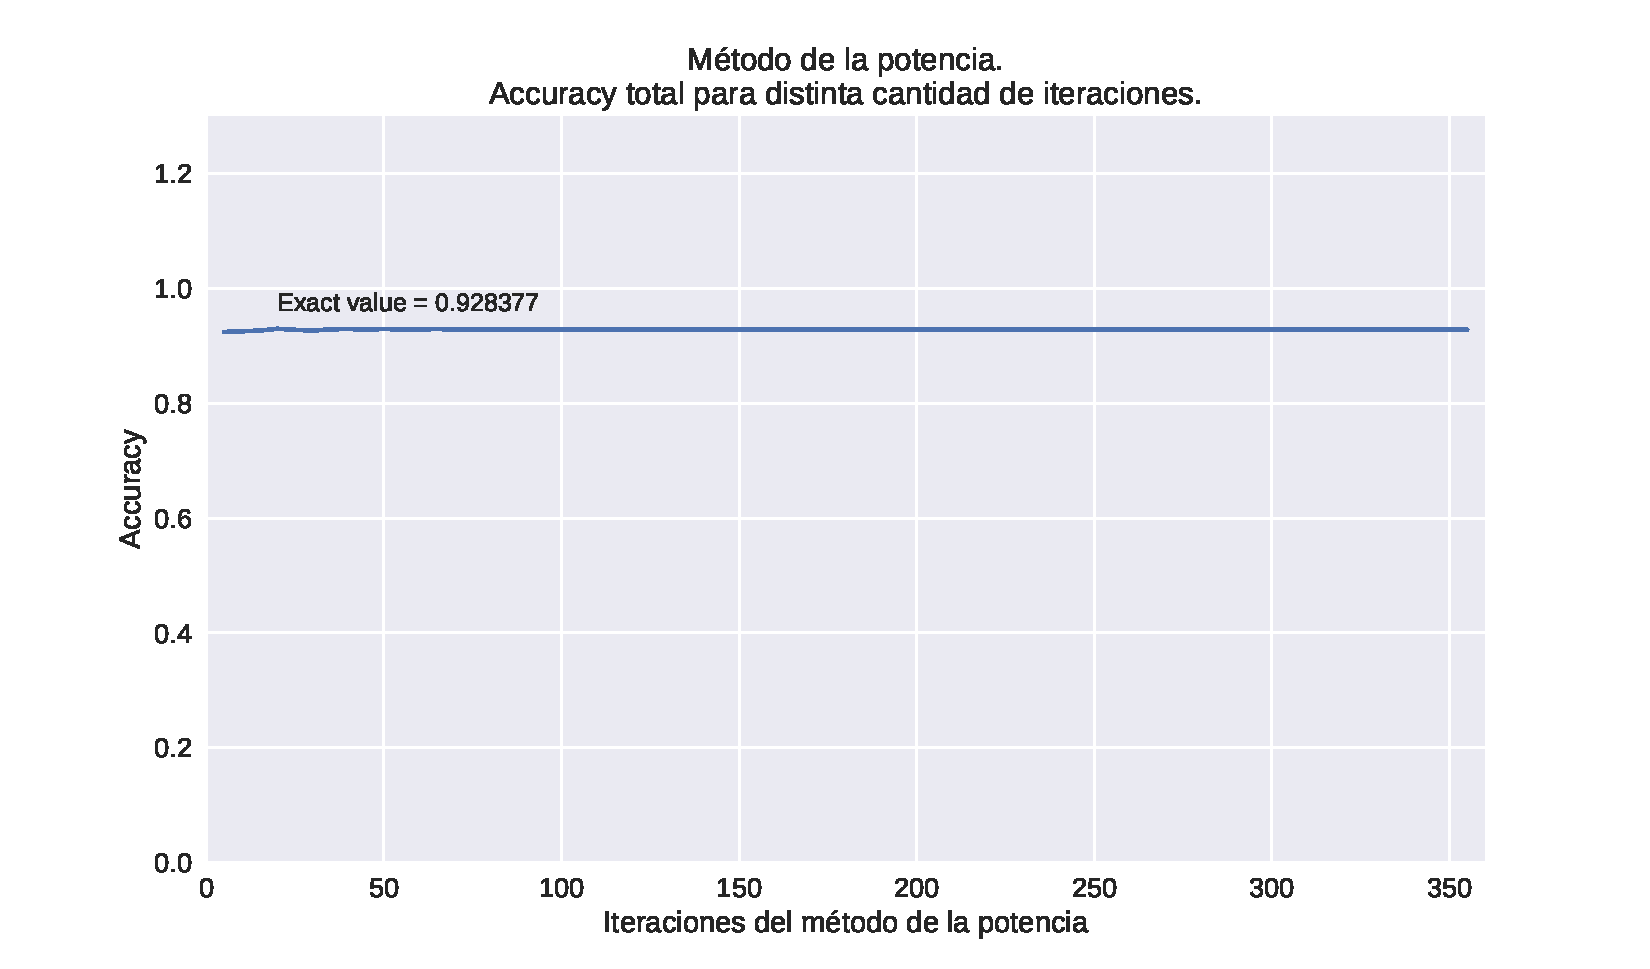
\includegraphics[scale=0.55]{informe/imagenes/potencia/accuracyPorIters.pdf} \\
    \captionof{figure}{Accuracy por cantidad de iteraciones. \\
    Todas las variables fijas \\ }
}
$ $\newline

Como podemos ver, la accuracy se mantiene constante, con la excepción de las cercanías de 10 iteraciones dónde aún son demasiado pocas. Consideramos que no es necesario tomar una cantidad de iteraciones demasiado alta, ya que con aproximadamente 50 parece ser más que suficiente. Es lógico pensar que a mayor cantidad de iteraciones, más tarda nuestro sistema en entrenar. Veamos si el incremento es significativo: \\

{\centering
    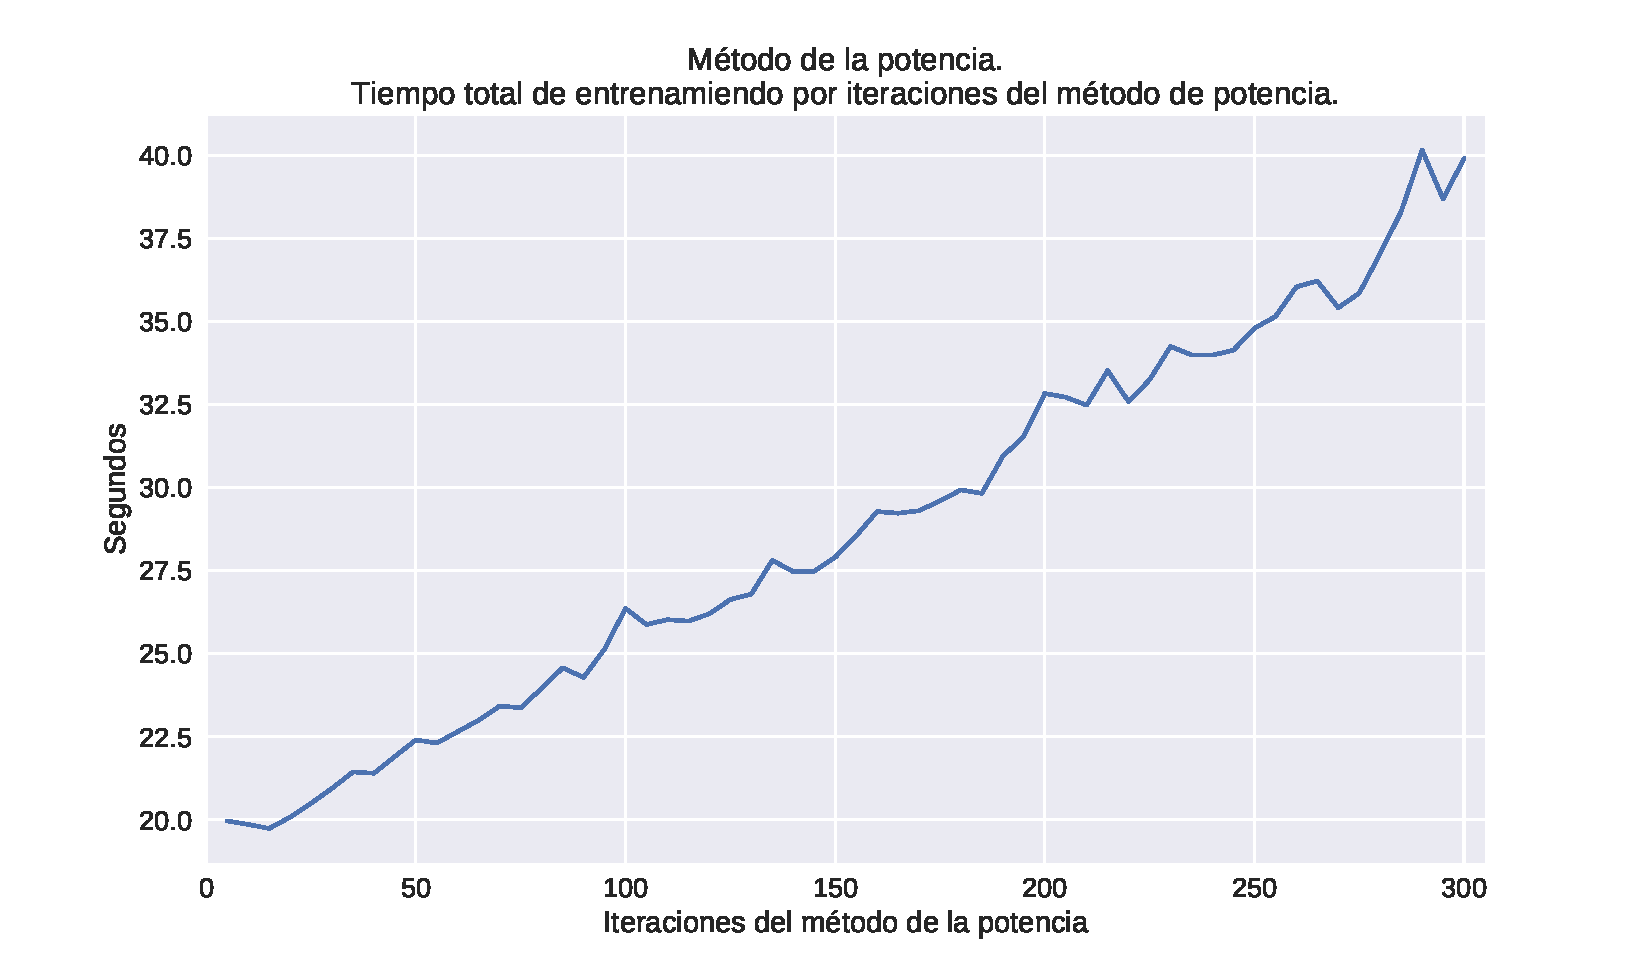
\includegraphics[scale=0.55]{informe/imagenes/potencia/tiempoPorIters.pdf} \\
    \captionof{figure}{Tiempo por cantidad de iteraciones. \\
    Todas las variables fijas \\ }
}
$ $\newline

La diferencia de tiempo es bastante notoria, sobre todo sabiendo que no estamos considerando la cantidad total de datos de entrenamiento. Dado que no encontramos diferencias de accuracy pero sí de tiempo, a partir de ahora fijaremos el parámetro de iteraciones en 50. \\

\section{Experimentación y resultados - kNN}

\subsection{kNN}

\todo[inline]{Quiza, graficar tiempos de knn para 10000 muestras, moviendo el k. Los datos ya estan tomados en knnMediciones, solo hay que extraerlos bien. Creo igual que conviene hacerlo en la comparacion con psa y ya, sino es info repetida-}

Nos gustaría analizar qué tan bien (o qué tan mal) se comporta kNN a medida que vamos variando el \textit{k}. Si bien nuestro espacio posible de muestras es 42000, usar un espacio de ese tamaño se vuelve prohibitivo ya que debemos iterar gran cantidad de veces sobre el espacio. Por este motivo, vamos a considerar un espacio de 10000 muestras. Es esperable que con las 42000 muestras consigamos resultados mejores, y lo verificaremos cuando enviemos los resultados a Kaggle. \\

Dado que nuestros vectores viven en $\mathbb{R}^{784}$, esperamos que los resultados aplicando kNN (sin reducir dimensiones) sean malos por problemas con la \textit{maldición de la dimensión}, y sobre todo porque no estamos considerando el espacio de muestras completo. \\

Sorprendentemente, lo que sucedió es todo lo contrario a lo que esperábamos, y con kNN obtuvimos (en promedio) precisiones de 0.95. \\

La mayoría de las clases se comportan de manera similar, salvo algunas excepciones que veremos más adelante. Veamos por ejemplo la clase del 0, que fue la \textit{mejor} clase.

{\centering
    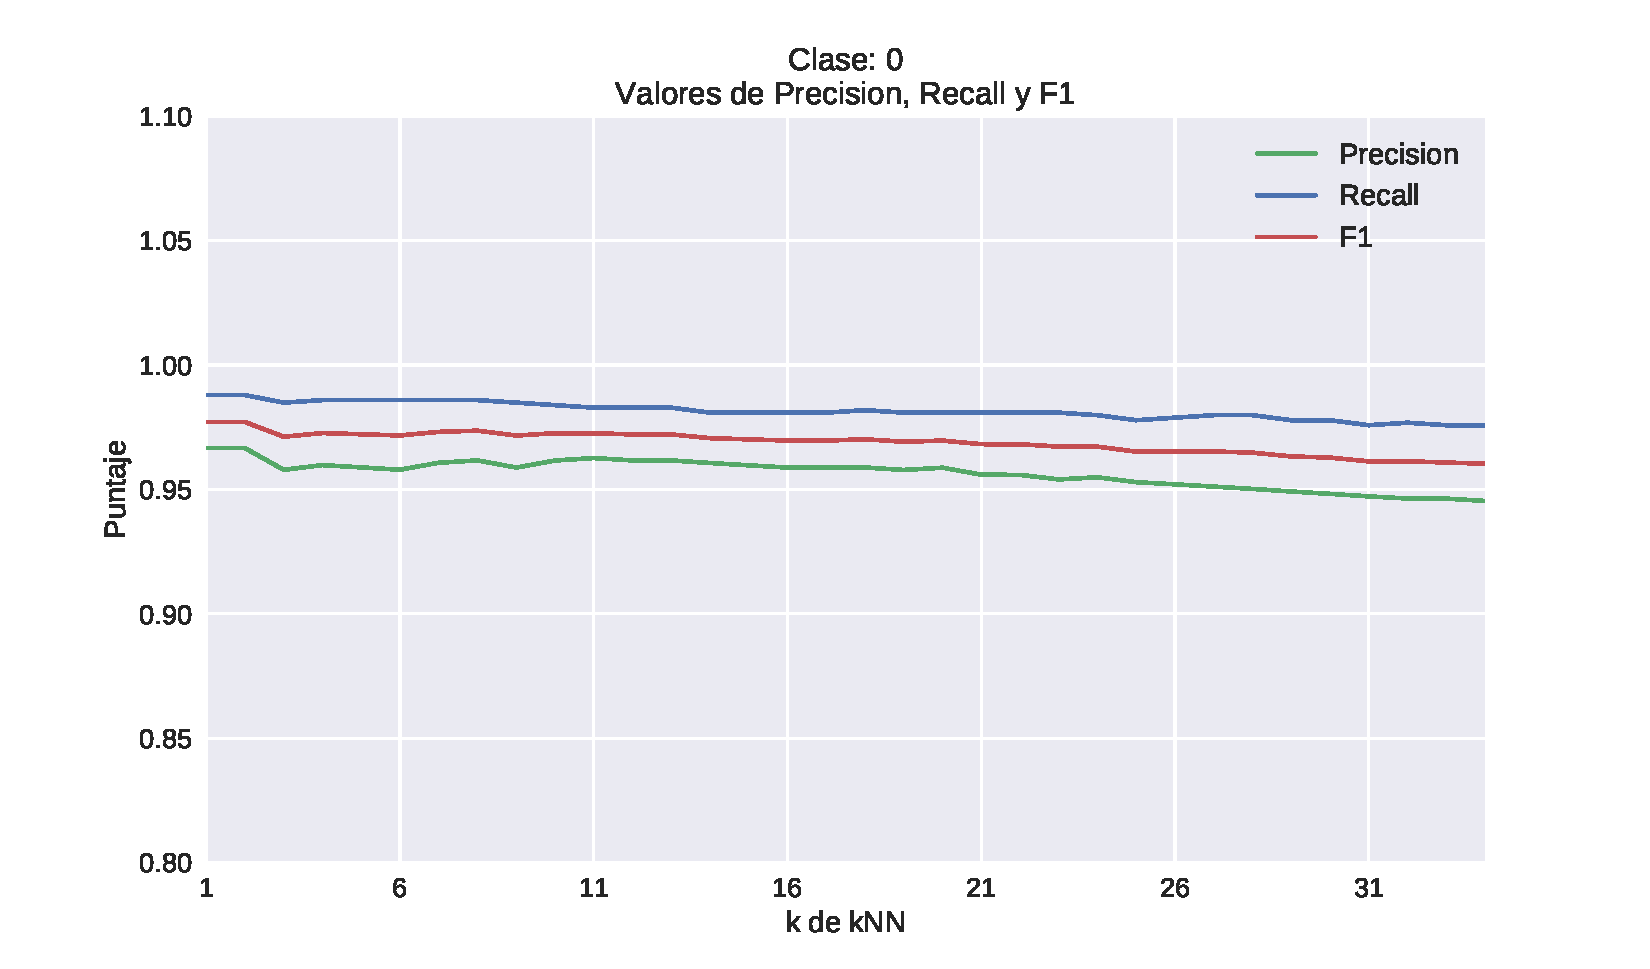
\includegraphics[scale=0.55]{informe/imagenes/knn/precisionClase0.pdf} \\
    \captionof{figure}{Clasificación para clase 0, sólo kNN.\\Precision, Recall y F1, variando k.\\}
}
$ $\newline

Dado que la mayoría de los gráficos son similares, sólo graficaremos a continuación aquellas clases que más se diferencian.

{\centering
    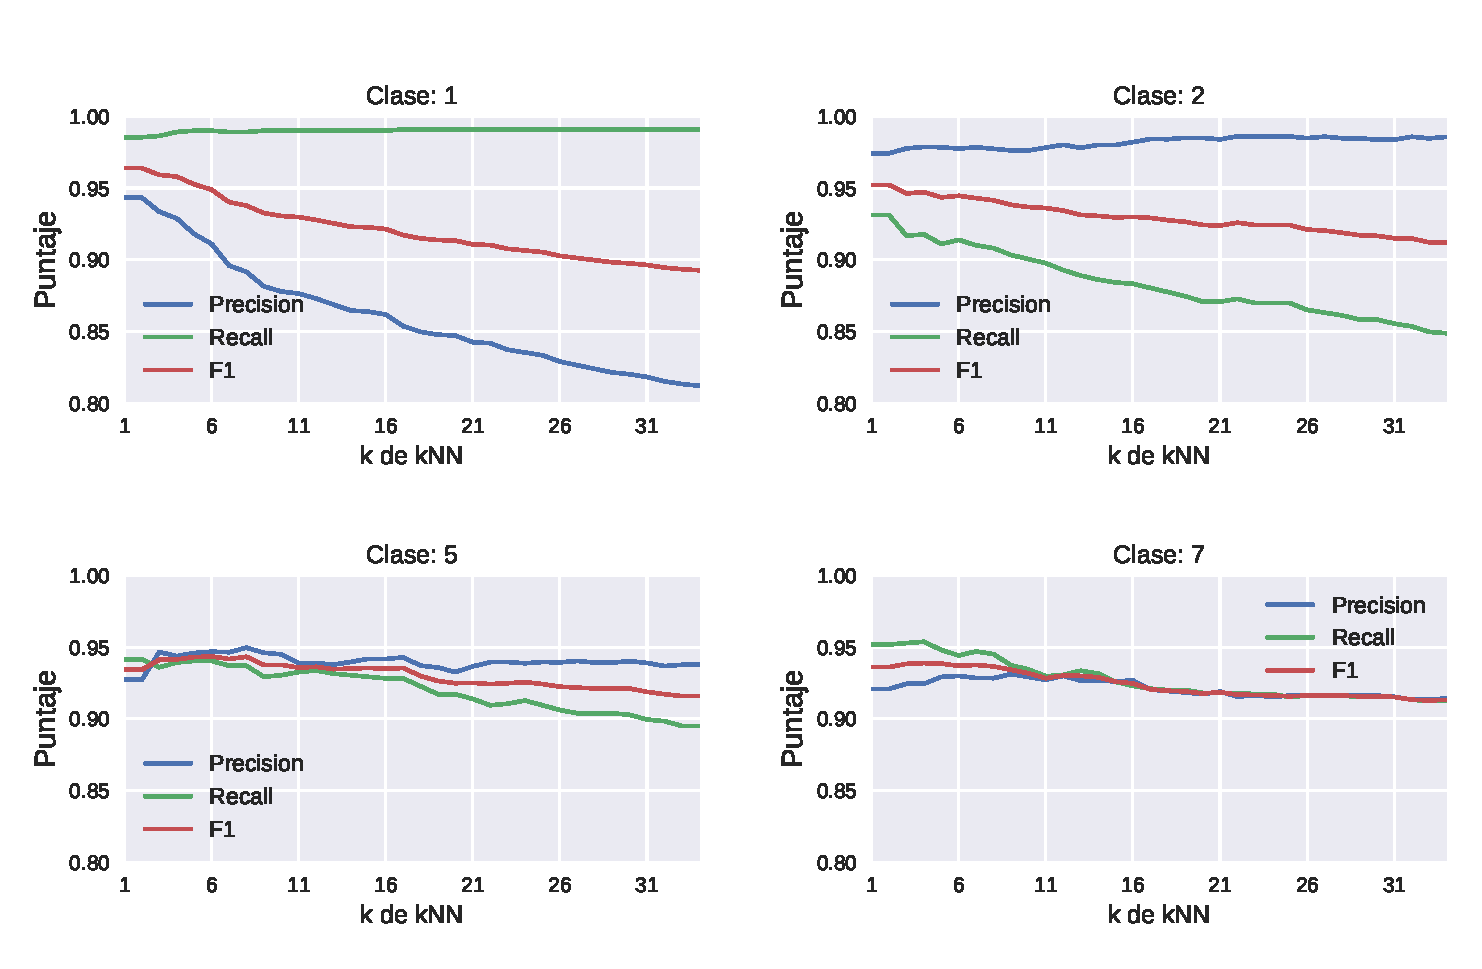
\includegraphics[scale=0.70]{informe/imagenes/knn/precisionClase1257.pdf} \\
    \label{fig:knnclasesvariacion}
    \captionof{figure}{Clasificación para clases 1, 2, 5 y 7, sólo kNN\\Valores de Precision, Recall y F1, variando k.\\}
}
$ $\newline

Lo primero que observamos es lo que nos sorprendió: todos comienzan con un Precision/Recall de aproximadamente 0.95, lo cual es un valor muy alto. Parece ser que pese a los problemas de dimensionalidad y del tamaño de la muestra, kNN se comporta bastante bien. Es esperable que con una muestra más grande se comporte mejor. Veremos más adelante qué dice Kaggle al respecto.\\

Otra cosa que podemos observar, es que a medida que el \textit{k} aumenta, \textit{en general} Precision y Recall disminuyen. Consideramos que este comportamiento tiene sentido ya que por el problema de la dimensionalidad, nuestros vectores estén muy dispersos, entonces con un \textit{k} mas grande los \textit{k} mas cercanos no necesariamente son los de su misma clase. \\

Algo destacable es lo que sucede con la clase del 1 y la clase del 2. Las curvas de Precision y de Recall son opuestas. Si categorizamos una imagen como un 2, es muy probable que sea un 2 realmente. Es decir, cuando lo categorizamos como un 2, no nos equivocamos. Sin embargo, hay muchas imágenes que realmente son 2 pero que no las categorizamos como tal. Con la clase del 1 nos pasa exactamente lo contrario. \\

El objetivo de el experimento era tratar de estimar el mejor \textit{k} para kNN. Nos concentraremos en la curva de F1, pues lo que nos interesa es tener un balance entre Precision y Recall. Buscamos el $k$ tal que F1 llegue a su máximo. Los siguientes son los valores obtenidos: \\

\begin{center}
    \begin{tabular}{| c | c | c | c | c | c | c | c | c | c | c |}
    \hline
    Clase   & 0 & 1 & 2 & 3 & 4 & 5 & 6 & 7 & 8 & 9  \\ \hline
    max_k       & 1 & 1 & 1 & 3 & 4 & 6 & 1 & 4 & 4 & 4  \\ \hline
    \end{tabular}
\end{center}

Sólo podemos quedarnos con un único k, y queremos \textit{favorecer} a todas las clases. Dado que el promedio es 2.9 y la mediana es 3, suponemos que el mejor k es 3.



\newpage


\subsection{K-Fold y Knn}

Al haber estimado el valor k de knn que mejor se comporta con las muestras de imágenes, nos propusimos analizar la cantidad de Folds con la que separamos nuestro espacio de muestra para entrenar.\\

Nuevamente utilizaremos 10000 de las 42000 imágenes, dado que, experimentar con distintos valores de kfolds se vuelve muy costoso mientras más cantidad de elementos haya. Consideramos que 10000 es un número representativo del total.\\

Como kfold es un método de corroborar estadísticamente el entrenamiento realizado, esperamos que los puntajes de cada clase no varíen demasiado conforme se vaya cambiando el K. \\

\begin{figure}[H]
\centering
  \subfloat{
   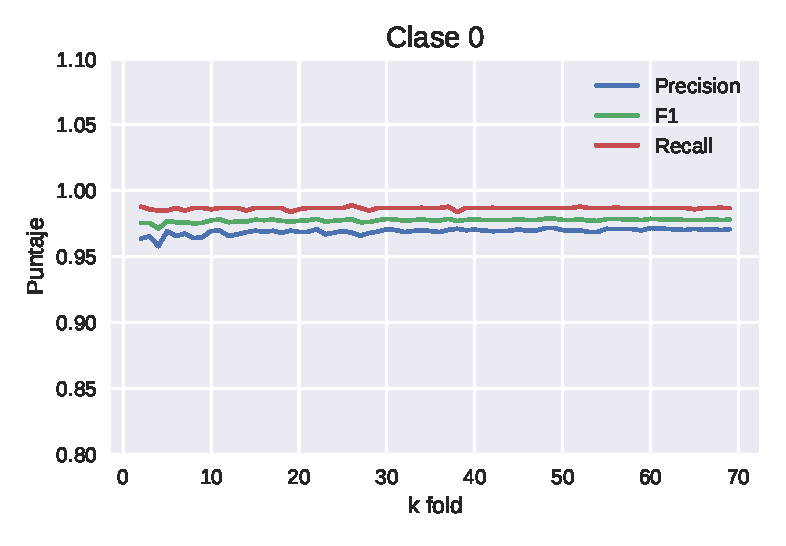
\includegraphics[width=0.5\textwidth]{informe/imagenes/kfold/knn/clase0.pdf}}
   \subfloat{
    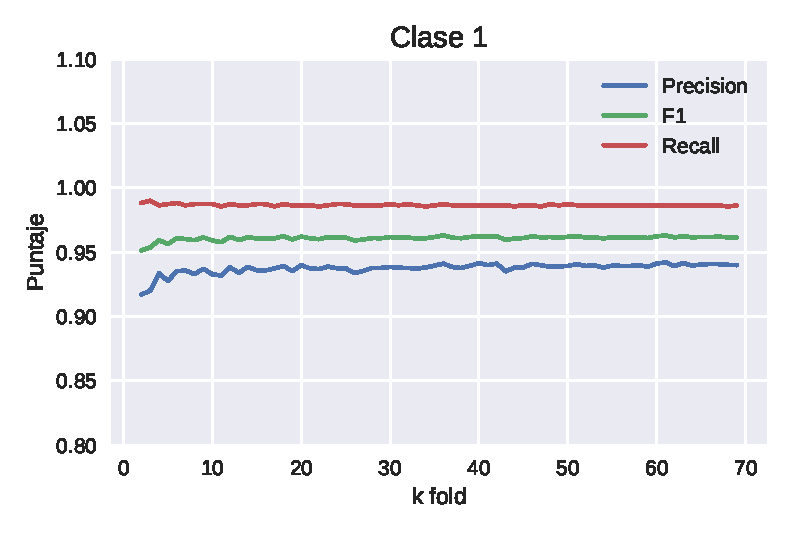
\includegraphics[width=0.5\textwidth]{informe/imagenes/kfold/knn/clase1.pdf}}

\centering
  \subfloat{
   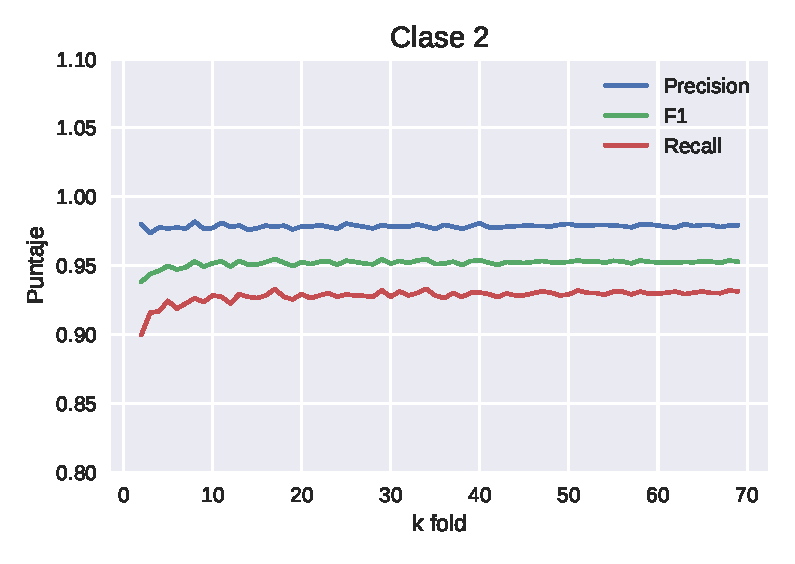
\includegraphics[width=0.5\textwidth]{informe/imagenes/kfold/knn/clase2.pdf}}
   \subfloat{
    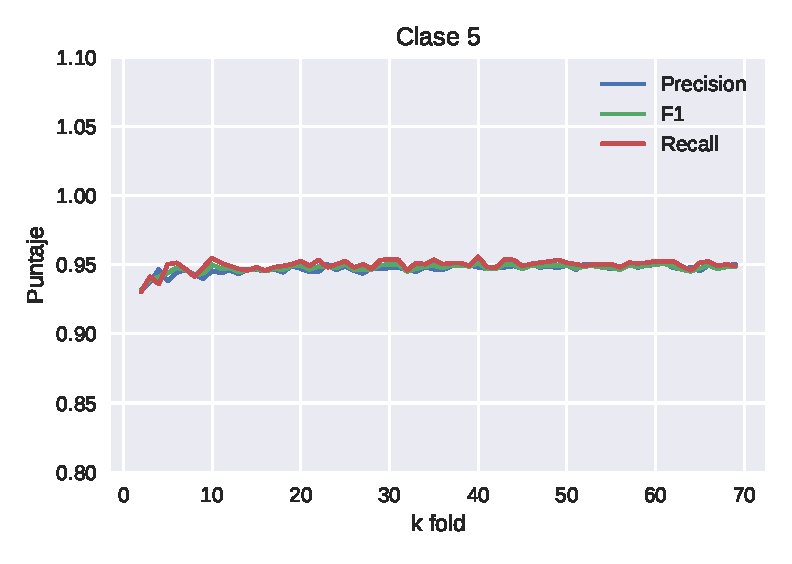
\includegraphics[width=0.5\textwidth]{informe/imagenes/kfold/knn/clase5.pdf}}

\centering
  \subfloat{

   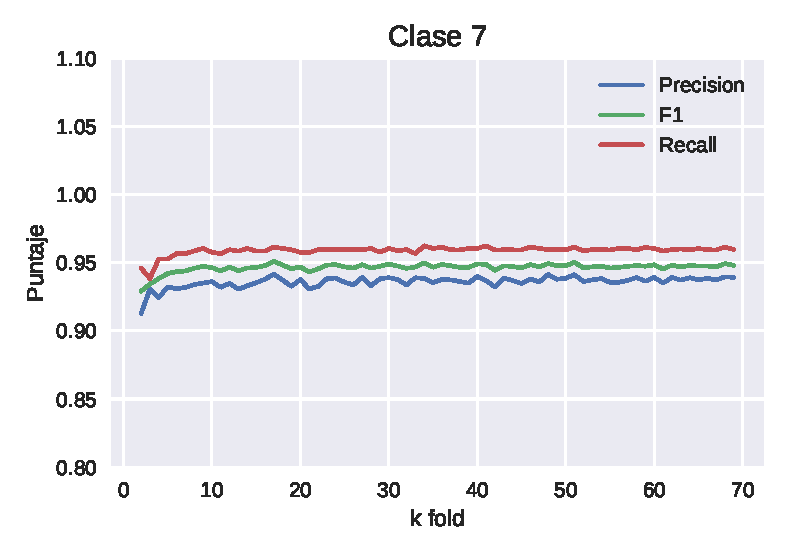
\includegraphics[width=0.5\textwidth]{informe/imagenes/kfold/knn/clase7.pdf}}
   \subfloat{

    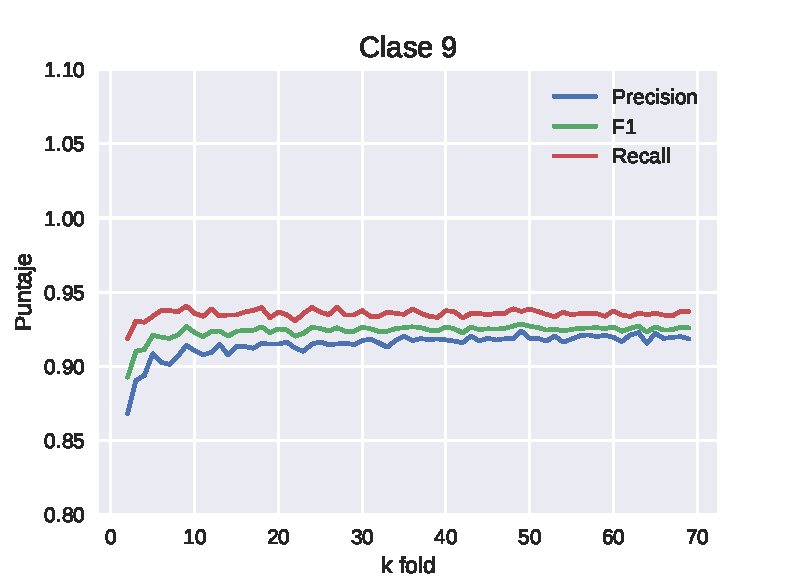
\includegraphics[width=0.5\textwidth]{informe/imagenes/kfold/knn/clase9.pdf}}

\captionof{figure}{Puntuaciones de las clases 0, 1, 2, 5, 7 y 9 a medida que aumenta el valor de K}
\end{figure}



Utilizamos K desde 2 hasta 70 porque creemos que abarcamos un rango amplio de valores.\\

Mostramos los gráficos de las clases 5, 7 y 9 porque son las más ``caóticas'' y de 0, 1 y 2 porque son standar, los gráficos de 3, 4, 6 y 8 son similares a estos últimos.\\

Si bien en algunas clases es más caótico que en otras, podemos observar que a medida que aumentamos los valores de K, el puntaje se estabiliza, lo cual no sucede con el tiempo que tarda al ejecutarse.\\

{\centering
    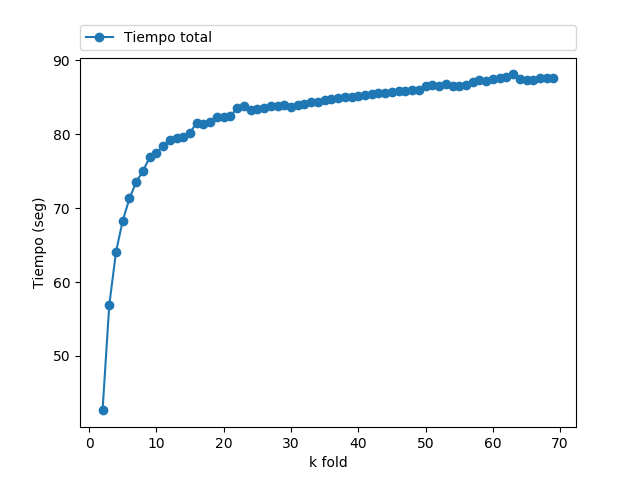
\includegraphics[scale=0.8]{informe/imagenes/kfold/knn/tiempokfold.png} \\
    \captionof{figure}{Tiempo de cómputo para cada K de K-Fold.\\}
}
$ $\newline

En este gráfico mostramos cuanto tarda en ejecutarse el entrenamiento con knn y utilizando la técnica kfold.\\

Por lo que consideramos que K=15 para kfold con knn es una buena estimación, dado que se mantienen altos los valores de los puntajes y el tiempo de cómputo es menor a lo que serían en caso de tomar un K mayor.\\



\newpage


















\subsection{Accuracy - Kaggle}

Como habíamos mencionado anteriormente, realizar el mismo experimento con el set completo de datos, sumado a las iteraciones por los folds, nos resulta demasiado costoso si consideramos una muestra demasiado grande. Es por esto que para comprobar la \textit{accuracy} de nuestro método decidimos probarlo directamente con la competencia de Kaggle. Queremos ver si efectivamente con k = 3 conseguimos el mejor resultado. Los siguientes resultados fueron obtenidos con un entrenamiento de las 42000 imágenes.\\

{\centering
    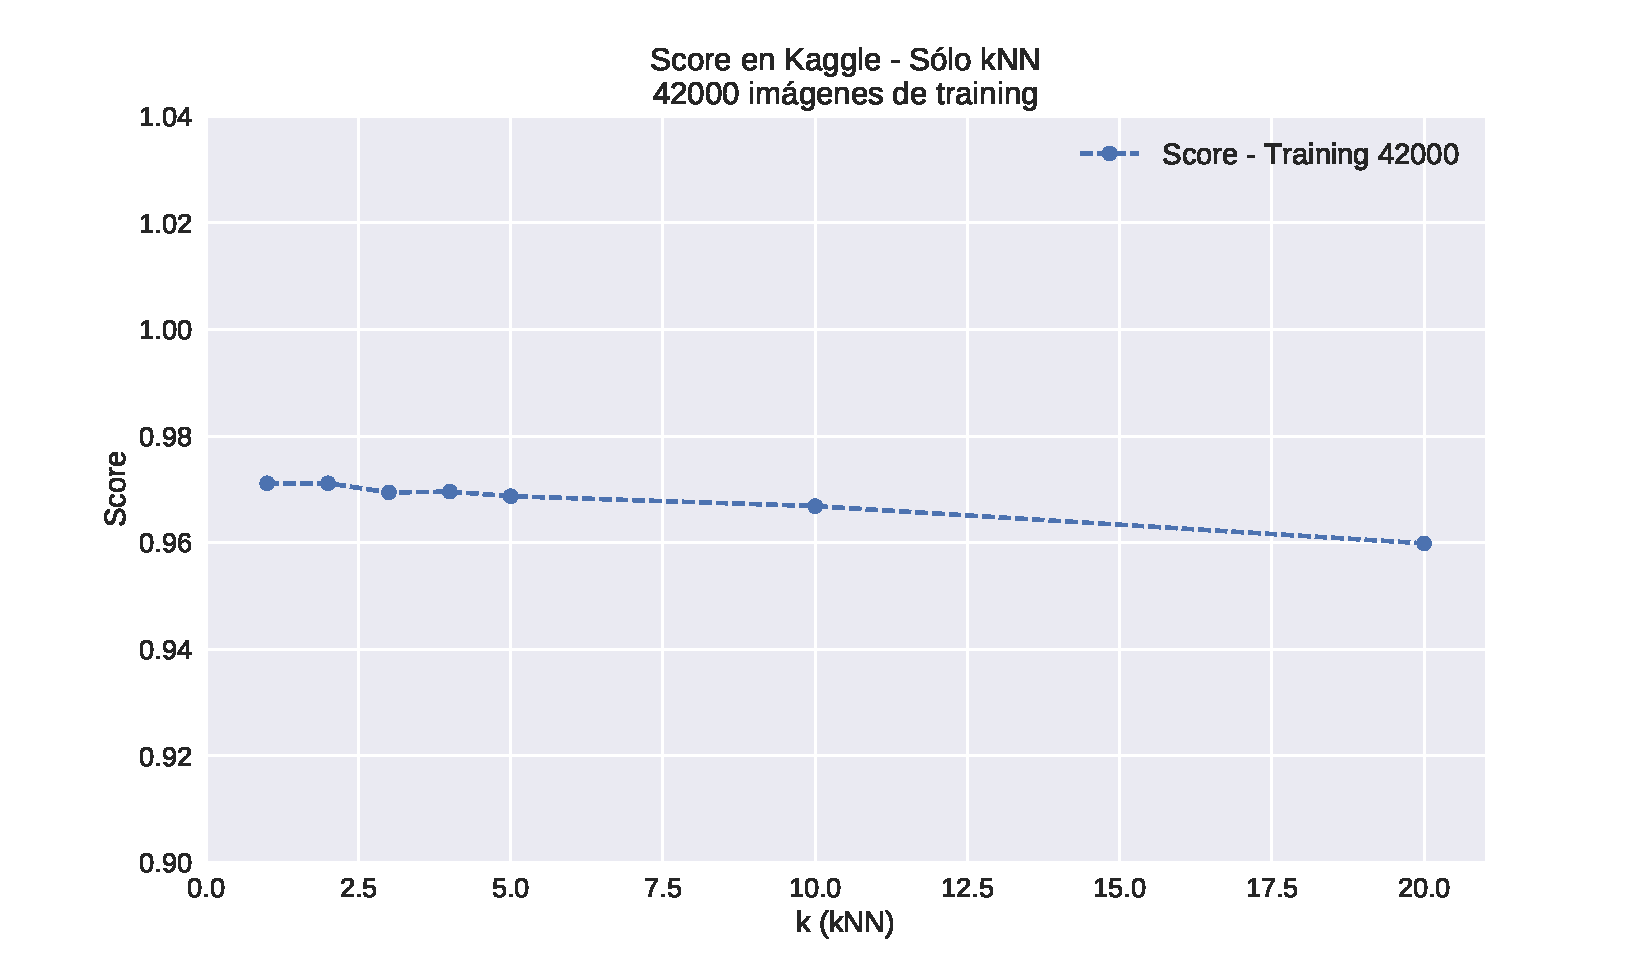
\includegraphics[scale=0.60]{informe/imagenes/knn/kaggleknn.pdf} \\
    \captionof{figure}{Accuracy en Kaggle variando k.\\Perfil del usuario utilizado: kaggle.com/jonnojs}
}
$ $\newline

Si bien nuestra predicción no fue perfecta, estuvo bastante cerca. Para una mejor apreciación de las diferencias, mostramos un cuadro comparativo con los 4 mejores resultados obtenidos, ordenados por score. \\

\begin{center}
    \begin{tabular}{| c | c |}
    \hline
    % k   & Score  \\ \hline
    % 2   & 0.97114  \\ \hline
    % 4   & 0.96957  \\ \hline
    % 3   & 0.96942  \\ \hline
     Accuracy    & k  \\ \hline
     0.97114  & 1  \\ \hline
     0.97114  & 2  \\ \hline
     0.96957  & 4  \\ \hline
     0.96942  & 3  \\ \hline
    \end{tabular}
\end{center}


En primer lugar, notar que k=1 y k=2 tienen el mismo puntaje. Esto es razonable, si consideramos que con k=2 las posibilidades sobre las clases del primer y segundo mas cercano son las siguientes: \\
\begin{itemize}
\item Si el primero es de clase X y el segundo es de clase X, entonces elegimos clase X
\item Si el primero es de clase X y el segundo es de clase Z, entonces igual nos quedamos con X pues fue el mas cercano.
\end{itemize}

Es decir, k=2 se comporta exactamente igual que no considerar ninguna vecindad. \\

Las diferencias de k=3 con k=2 y k=4 son 0.00172 y 0.00015 respectivamente, que es bastante pequeña considerando la reducción de muestras que hicimos. \\

Aunque los números no mienten, no nos parece intuitivo que no considerar ninguna vecindad sea la mejor opción. Imaginamos que este resultado puede asociarse con la maldición de la dimensionalidad, y creemos que con PCA el mejor k será uno mayor. También es posible que los datos de tests de Kaggle tengan un sesgo hacia aquellos cuyos $k$ óptimo es menor, pero como no conocemos las verdaderas etiquetas no podemos saberlo. \\

% \todo[inline]{¿QUIZA? -> Concluimos que para unicamente kNN, el mejor parámetro para k es k=EQUIS.}

\section{Experimentación y resultados - PCA}

\subsection{PCA}

En esta sección intentaremos estimar los mejores parámetros para el método de PCA. Debido a que el tiempo de procesamiento es menor que en kNN, pudimos realizar los experimentos con la base completa de 42000 imágenes, por lo que es esperable que obtengamos resultados de mejor calidad. De todas maneras, en Kaggle enviamos resultados tanto de kNN como PCA que utilizaban la misma cantidad de imágenes de entrenamiento, por lo que ambos métodos estarán en igualdad de condiciones en ese caso al determinar cuál resultó mejor. \\

Dado que lo que nos interesará para determinar los mejores parámetros será el balance entre Precision y Recall, consideraremos los valores de F1 para nuestro análisis.  \\

El siguiente es un gráfico de F1 para algun valor de \textit{alpha} a modo de ejemplo, variando el $k$. Elegimos para mostrar las mismas clases que mostramos en la sección de kNN (1, 2, 5, 7) para tener una primer idea cómo se comporta nuestro método. Recordemos que en kNN para esas clases, los resultados eran los que tenían mayor variación. \\

{\centering
    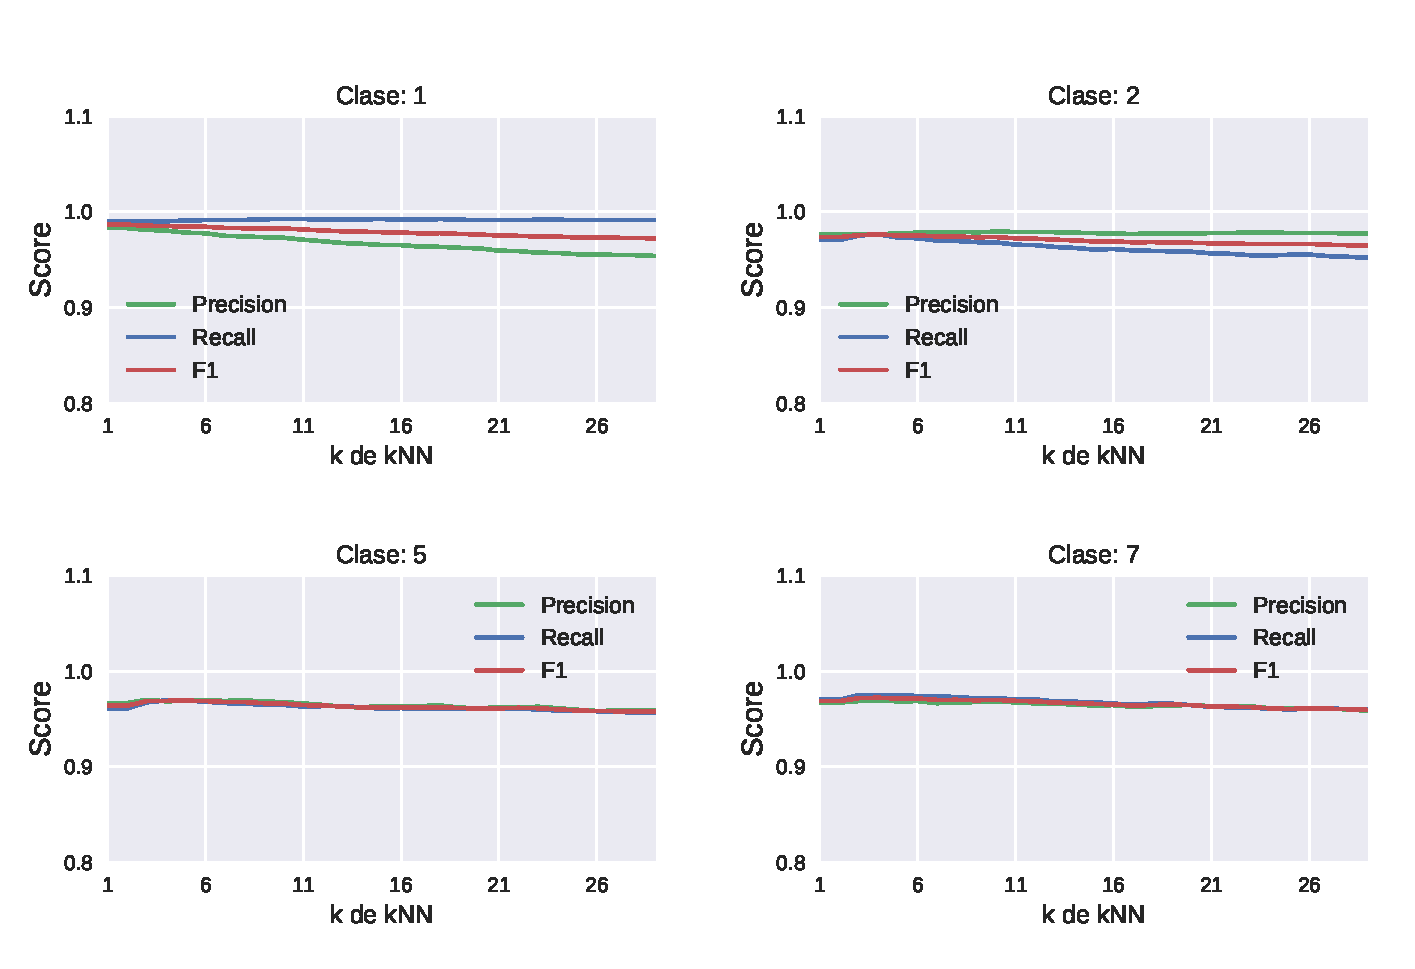
\includegraphics[scale=0.65]{informe/imagenes/pca/variacionKClases1257PresRecall.pdf} \\
    \captionof{figure}{Scores de clasificación para clases 1, 2, 5 y 7, con variación de k. Alpha=30 fijo.}
}
$ $\newline

Lo que notamos en primer lugar es la similitud entre las clases. Mientras que con sólamente kNN las curvas se veían muy dispares (Ver Figura en~\ref{fig:knnclasesvariacion}) aquí podemos observar que PCA es bastante estable cuando consideramos diferentes clases. Lo segundo a notar es que con $k$ cercano a 4, los scores tienen un \textit{pequeño} salto positivo. Si bien esto es para un \textit{alpha} particular, esto es algo que se repite para diferentes valores de \textit{alpha}. Como adelantamos, nos interesará considerar el balance entre Precision y Recall, así que sólo mostraremos F1 para no sobrecargar los gráficos. \\

{\centering
    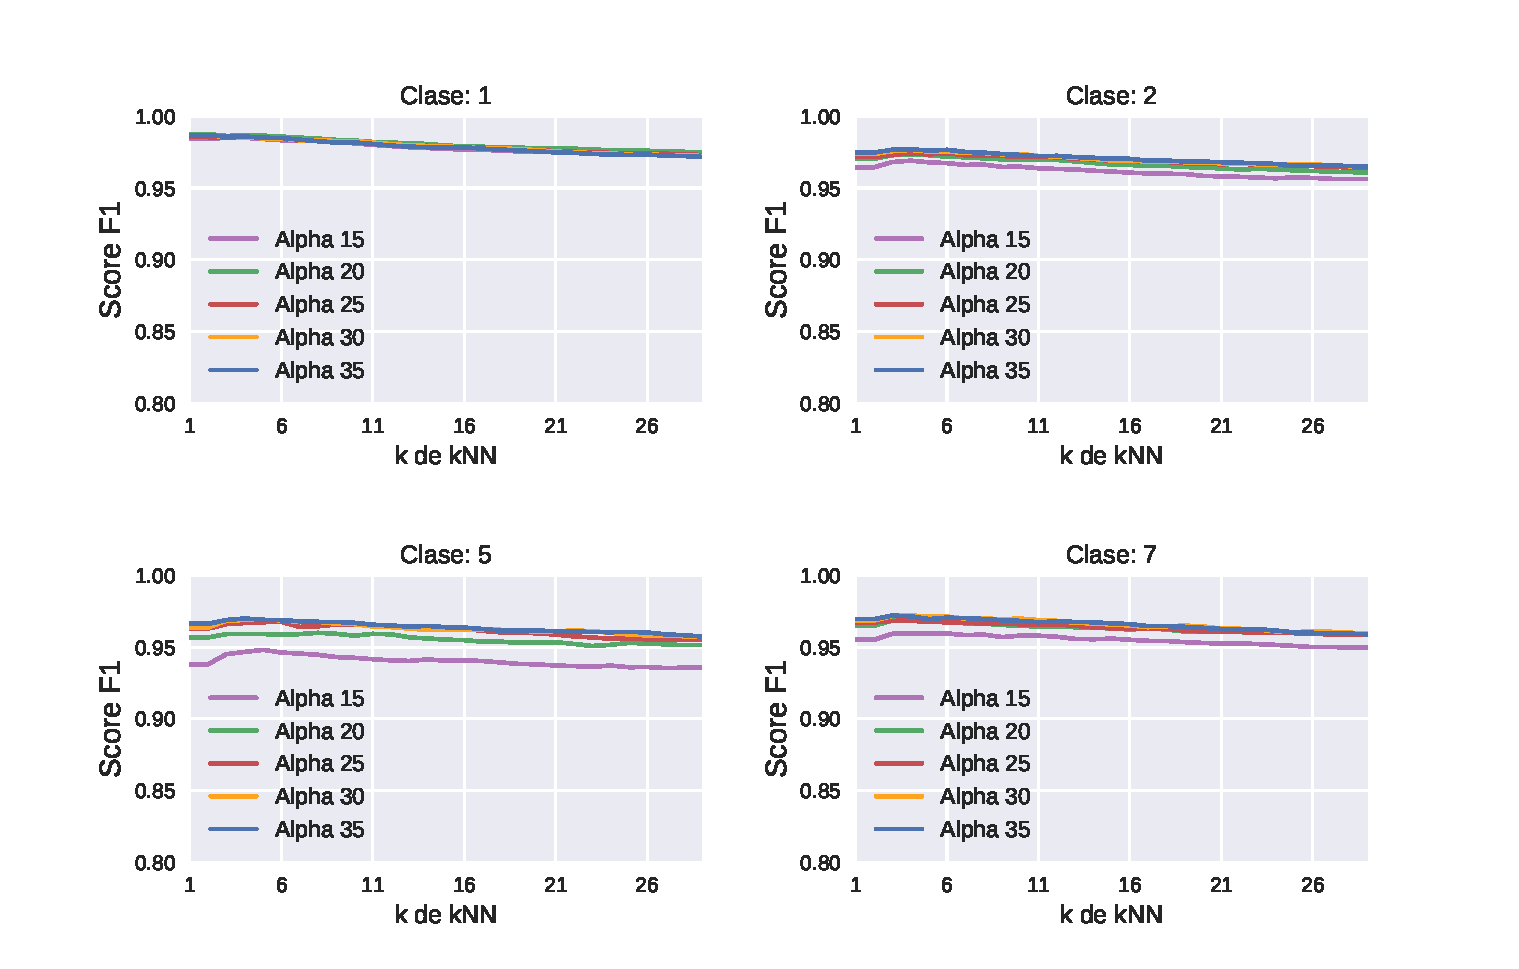
\includegraphics[scale=0.65]{informe/imagenes/pca/variacionKClases1257.pdf} \\
    \captionof{figure}{Clasificación según F1 para clases 1, 2, 5 y 7, con variación de k.}
}
$ $\newline

Vemos que la tendencia del mejor $k$ es cercano a 4 se mantiene. No estamos mostrando el gráfico para las demás clases (que se ven extremadamente similares) pero mas allá del gráfico, tenemos los datos reales. Tomando promedios (para cada clase) variando \textit{alpha}, obtuvimos que el mejor $k$ es $k=4$ en muchas de las clases, y $k=5$ para otras. Si bien por poco margen, $k=4$ tiene mayoría así que será el $k$ elegido. Dependiendo cómo están distribuidos los datos, es posible que esto no siempre sea el mejor, sin embargo creemos que es la mejor aproximación. \\

Ya tenemos fijo $k$, queremos determinar $alpha$. Para esto dejemos fijo $k=4$. Lo que esperamos obtener es una mejora de score a medida que aumentemos el $alpha$, pues cuántas mas componentes consideremos, más precisios deberían ser las clasificaciones. \\

Creemos que no tiene demasiado sentido mostrar los gráficos de las 10 clases pues son muy similares, así que continuemos con las 4 clases tomadas anteriormente. Los resultados obtenidos son los siguientes: \\

{\centering
    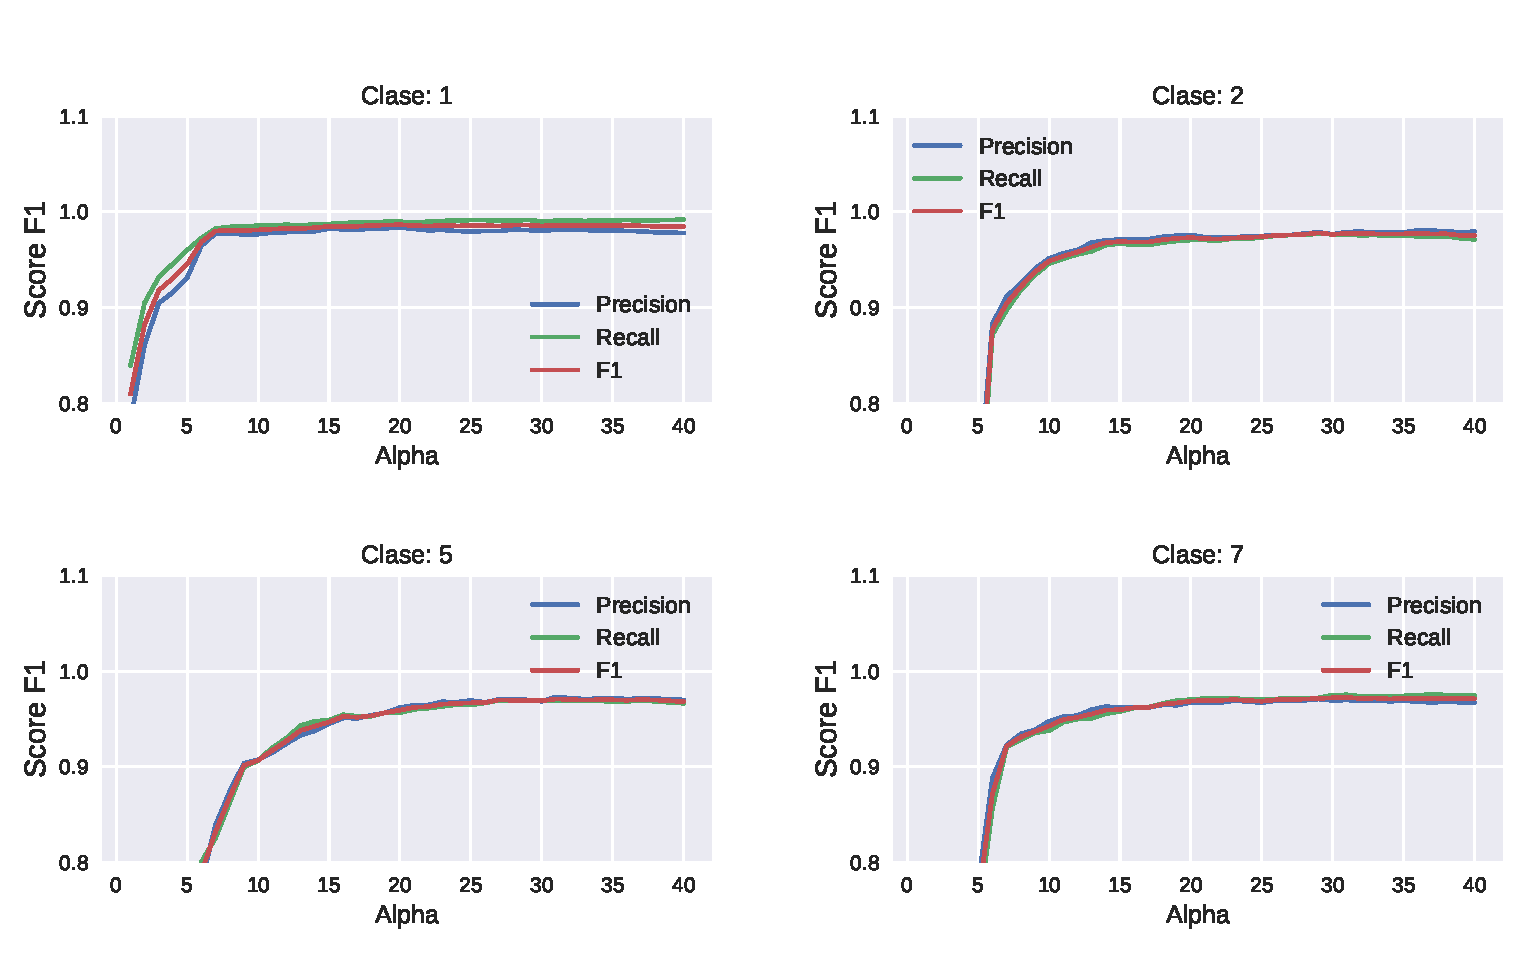
\includegraphics[scale=0.65]{informe/imagenes/pca/variacionAlphaClases1257KFijo.pdf} \\
    \captionof{figure}{Score de clasificación para clases 1, 2, 5 y 7, con variación de alpha.}
}
$ $\newline

Algo que nos sorprendió es la velocidad con la cual se alcanza el máximo valor. Con aproximadamente 15 componentes principales ya se logra una efectividad comparable con kNN simple (728 componentes). \\

Podemos observar que a partir de $alpha=25$ el score se estabiliza y se mantiene casi constante. Es aproximadamente para $alpha=40$ cuando empieza una \textit{muy leve} disminución del score, y las curvas de precision y recall comienzan a separarse. Lo esperable es que cuando $alpha$ sea demasiado grande el score disminuya aún mas, pues caemos nuevamente en la maldición de la dimensionalidad. Si bien sería interesante comprobarlo experimentalmente, no pudimos realizar el experimento. \\

Utilizando los datos reales, calculamos el mejor $alpha$ para cada clase, y promediamos los resultados. Obtuvimos que (tanto con $k=4$ como con $k=5$) el óptimo se alcanza con $alpha=31$. \\


\subsection{Accuracy - Kaggle}

Tal como hicimos con el método de kNN, nos gustaría ver cuáles son los resultados de PCA en la competencia de Kaggle. Con esto esperamos obtener el accuracy para nuestro método con un set de datos para el cual no conocemos sus etiquetas, que no fue utilizado como parte del entrenamiento. Nos parece la mejor opción para medir la efectividad pues es lo más cercano que tenemos al ambiente fuera de nuestro entorno de pruebas. \\

Nos gustaría ver, además, si el $alpha$ estimado se corresponde con el $alpha$ máximo en Kaggle. Creemos que en el caso de no ser exacto, estaremos muy cerca ya que nuestra recolección de datos sobre precision y recall fue bastante detallada. En el gráfico a continuación se muestran los resultados para diferentes $alpha$, siempre con $k=4$. \\

{\centering
    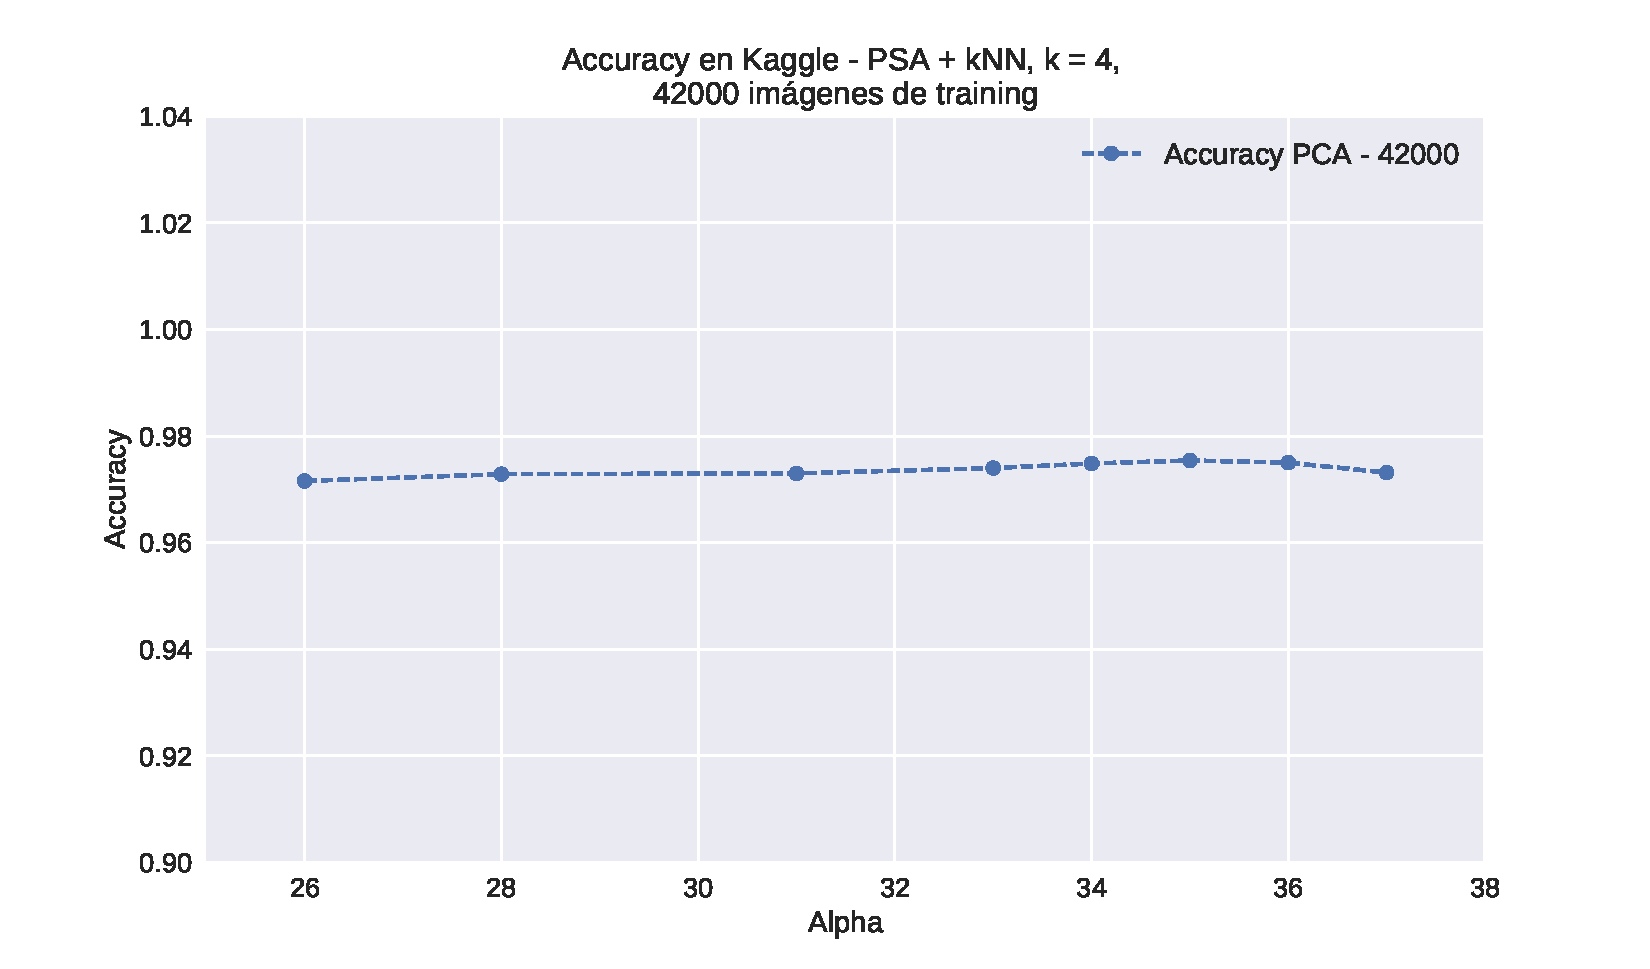
\includegraphics[scale=0.60]{informe/imagenes/pca/clasificacionKaggle.pdf} \\
    \captionof{figure}{Accuracy en Kaggle variando alpha.\\Perfil del usuario utilizado: kaggle.com/jonnojs}
}
$ $\newline

Veamos los datos exactos de los 3 máximos puntajes comparados con nuestra predicción: \\

\begin{center}
    \begin{tabular}{| c | c |}
    \hline
    % k   & Score  \\ \hline
    % 2   & 0.97114  \\ \hline
    % 4   & 0.96957  \\ \hline
    % 3   & 0.96942  \\ \hline
     Accuracy    & Alpha  \\ \hline
     0.97542  & 35  \\ \hline
     0.97500  & 36  \\ \hline
     0.97485  & 34  \\ \hline
     % ..  & ..  \\ \hline
     0.97300  & 31  \\ \hline
    \end{tabular}
\end{center}

La diferencia entre $alpha=31$ con el máximo es 0.00242. Es decir, nuestra predicción estuvo \textit{bastante cercana} pero no fue del todo precisa. Para descartar que sean diferencias producidas por la elección de $k$, se relizaron algunas pruebas con $k=3$ y $k=5$, y en todas se obtuvo un puntaje superio usando $k=4$. Concluimos que en Kaggle los mejores parámetros para PCA son $k=4$ y $alpha=35$.  \\

\section{Experimentación - Tiempo}

Para cerrar con nuestra experimentación, queremos mostrar una comparación entre ambos métodos con respecto al tiempo de ejecución. \\

En kNN, cada vez que comparamos dos vectores debemos analizar 728 componentes, mientras que con PCA nos basta con analizar alrededor de 30 componentes. Esto nos dá la pauta que la clasificación será mucho mas rápida con el segundo método. Sin embargo, en PCA tenemos el costo adicional de crear la matriz de covarianza y diagonalizarla, que no algo manor. Entonces la pregunta que nos hacemos es, ¿esto \textit{compensa} los costos de alguna manera? ¿Cuál sera mas rápido? \\

En las mediciones tomadas, los $k$ y $alpha$ están fijos en ambos métodos. Las diferencias temporales que podrían surgir por la elección de estos parámetros son constantes en el límite, por lo que al ir aumentando la cantidad de imágenes dejan de tener relevancia. Los tiempos no se obtuvieron en una única pasada, sino que ejecutamos los métodos varias veces y lo que graficamos es el promedio obtenido. \\

Como nota del experimento, fuimos aumentando la cantidad de imágenes total y esto implica que lo que aumenta es la cantidad usada como entrenamiento y \textit{también} la cantidad para clasificar. Es decir, lo que se mide es el tiempo tanto de entrenamiento como de clasificación. Los siguientes fueron los resultados. \\

{\centering
    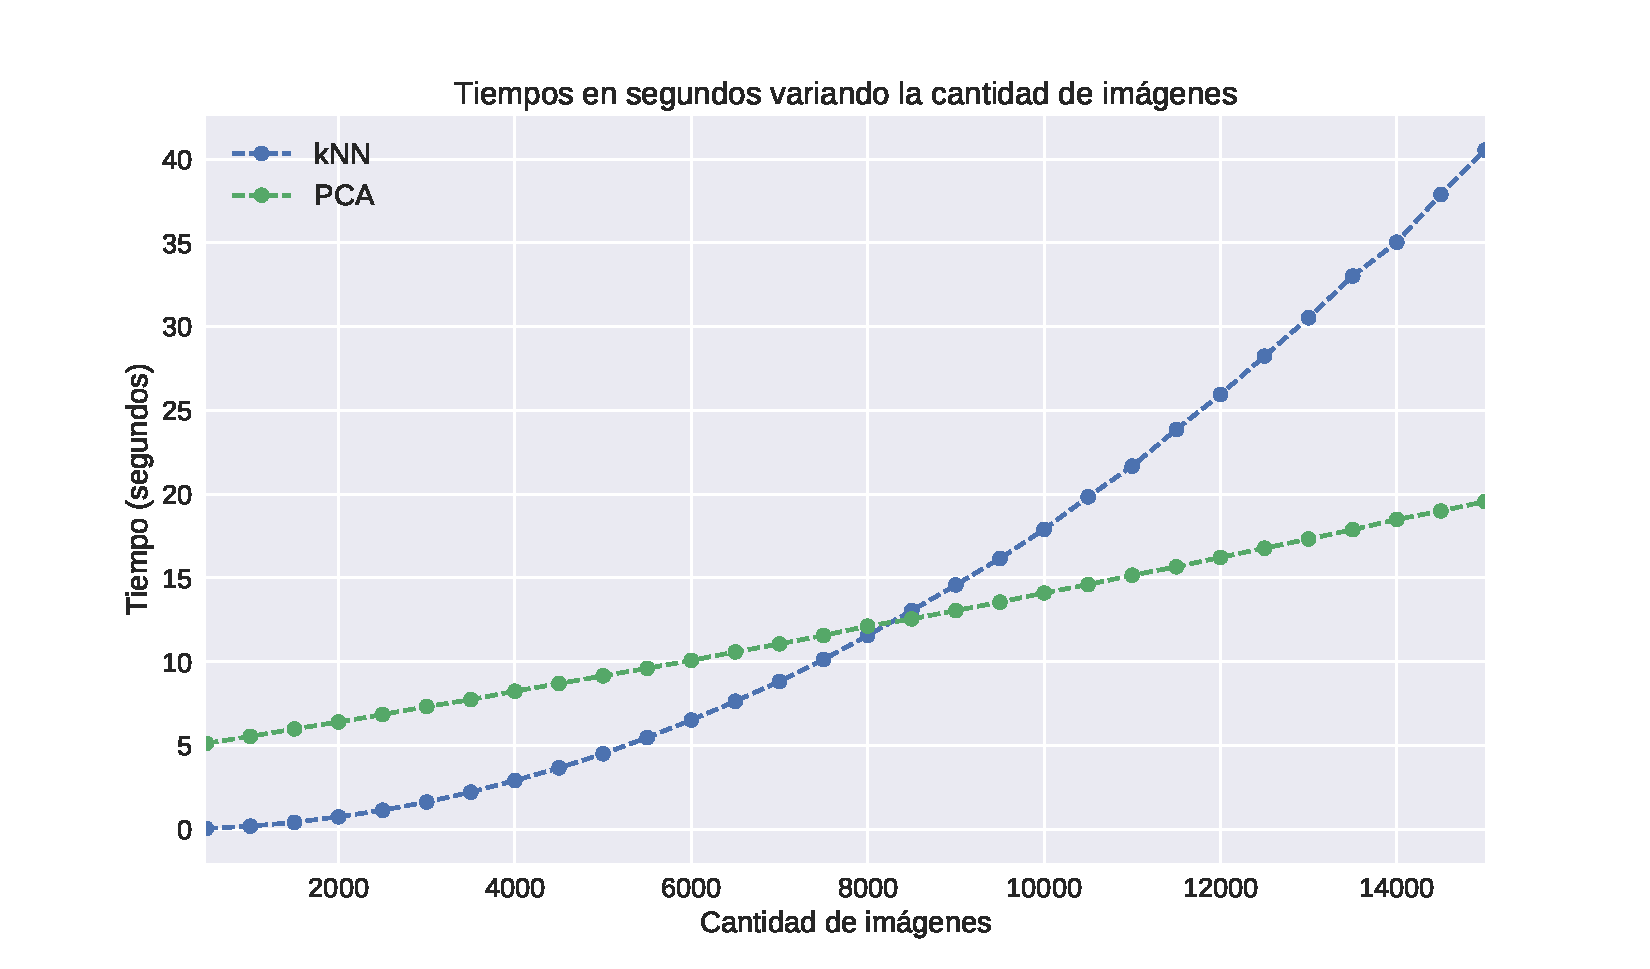
\includegraphics[scale=0.60]{informe/imagenes/tiemposKnnVsPsa.pdf} \\
    \captionof{figure}{Tiempos promedio para ambos métodos, variando la cantidad de imágenes.}
}
$ $\newline

Aquí vemos el resultado final. Para conjuntos pequeños de imágenes kNN es claramente más rápido. Esta diferencia inicial la explicamos por el tiempo de entrenamiendo de PCA, dónde contruir la matriz de covarianza y diagonalizar tiene un costo asociado. Sin embargo, los resultados con pacas imágenes no son interesantes, pues los entrenamientos con la mayor cantidad de datos posibles son los que logran mejores resultados. \\

A medida que la cantidad de imágenes va aumentando, la curva de tiempo de kNN crece con mayor velocidad, lo cual explica nuestra dificultad para trabajar con conjuntos grándes de imágenes. Con PCA esto no sucede, y de hecho hemos podido realizar nuestros experimentos con el conjunto completo de 42000 muestras sin mayores dificultades. Dado que lo deseable es realizar entrenamientos con cantidades grandes de imágenes, concluimos que PCA es el que tiene el mejor costo computacional. \\

No queremos dejar del lado el hecho de que, más allá de la estimación de los parametros, obtuvimos un accuracy de 0.97542 utilizando PCA. Quedamos muy conformes ya que nos parece un número muy alto, que supera ampliamente las expectativas que teníamos. \\

Recordemos que con kNN obtuvimos un accuracy máximo de 0.97114. Es decir, con PCA obtuvimos \textbf{mejores} resultados (Exactamente una diferencia de 0.00428). La ganancia no fue únicamente en efectividad, sino que tambien en costo computacional. Con estas últimas dos observaciones, estamos en condiciones de asegurar que PCA es el mejor de ambos métodos. \\
